\documentclass[10pt,aspectratio=43,mathserif]{beamer}
%\usepackage{nju}			 %导入 nju 模板宏包
%\usepackage[UTF8]{ctex}      %导入 ctex 宏包,添加中文支持
\usepackage{xeCJK}
\usepackage{amsmath,amsfonts,amssymb,bm}   %导入数学公式所需宏包
\usepackage{color}			 %字体颜色支持
\usepackage{graphicx,hyperref,url}
\usepackage{listings}
\usepackage{booktabs}
\usepackage{multirow}
\usepackage{float}
\usepackage{mhchem}
\usepackage{animate}
\usepackage[isbn=false,doi=false,uniquename=init]{biblatex}
\addbibresource{icc_pre_1108.bib}
\AtEveryCitekey{\clearfield{title}}
\AtEveryBibitem{\clearfield{title}}
\usepackage{textcomp}
\usepackage{multicol}

%\beamertemplateballitem		%设置 Beamer 主题
%\catcode`\。=\active        %或者=13
%\newcommand{。}{.}         %将正文中的“。”号转换为“.”。

%\AtBeginSection[]
%{
%  \begin{frame}
%    \frametitle{Contents}
%    \tableofcontents[currentsection]
%  \end{frame}
%}



\title{Homework Report}	        %首页信息设置

\author[]{            %个人信息设置
    Shirong Wang\\[0.3cm]
    %15XXXXXXXX\\[0.3cm]
    Kuang Yaming Honors School}

\date{\today}



\begin{document}

\begin{frame}
\titlepage
\end{frame}

%\begin{frame}
%\frametitle{Contents}
%\tableofcontents
%\end{frame}

\section{Reaction I}
\begin{frame}
\frametitle{Oxidative addition of $ \ce{Pt(PMe_3)_2} $}
\begin{equation}\label{key}
\ce{Pt(PMe_3)_2 + H_2 -> Pt(PMe_3)_2H_2}
\end{equation}

\end{frame}

\begin{frame}
\textbf{Question:} \textsl{cis} or \textsl{trans} product?\\

\begin{figure}[H]
	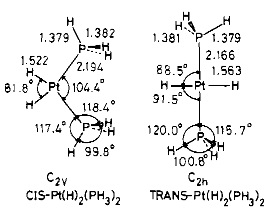
\includegraphics[width=0.45\linewidth]{Pt1.jpg}
\end{figure}
Only \textsl{cis} product is symmetry allowed. (\textsl{cis} product can be converted into \textsl{trans}, although)\\

\fullcite{Kitaura1981}
%\nocite{Kitaura1981}
%\printbibliography
\end{frame}

\begin{frame}
\frametitle{TS}
\begin{figure}
	\animategraphics[width=0.45\linewidth,loop,autoplay]{30}{../Pt/pbe0/vib/Pt_tsb000}{00}{47}
	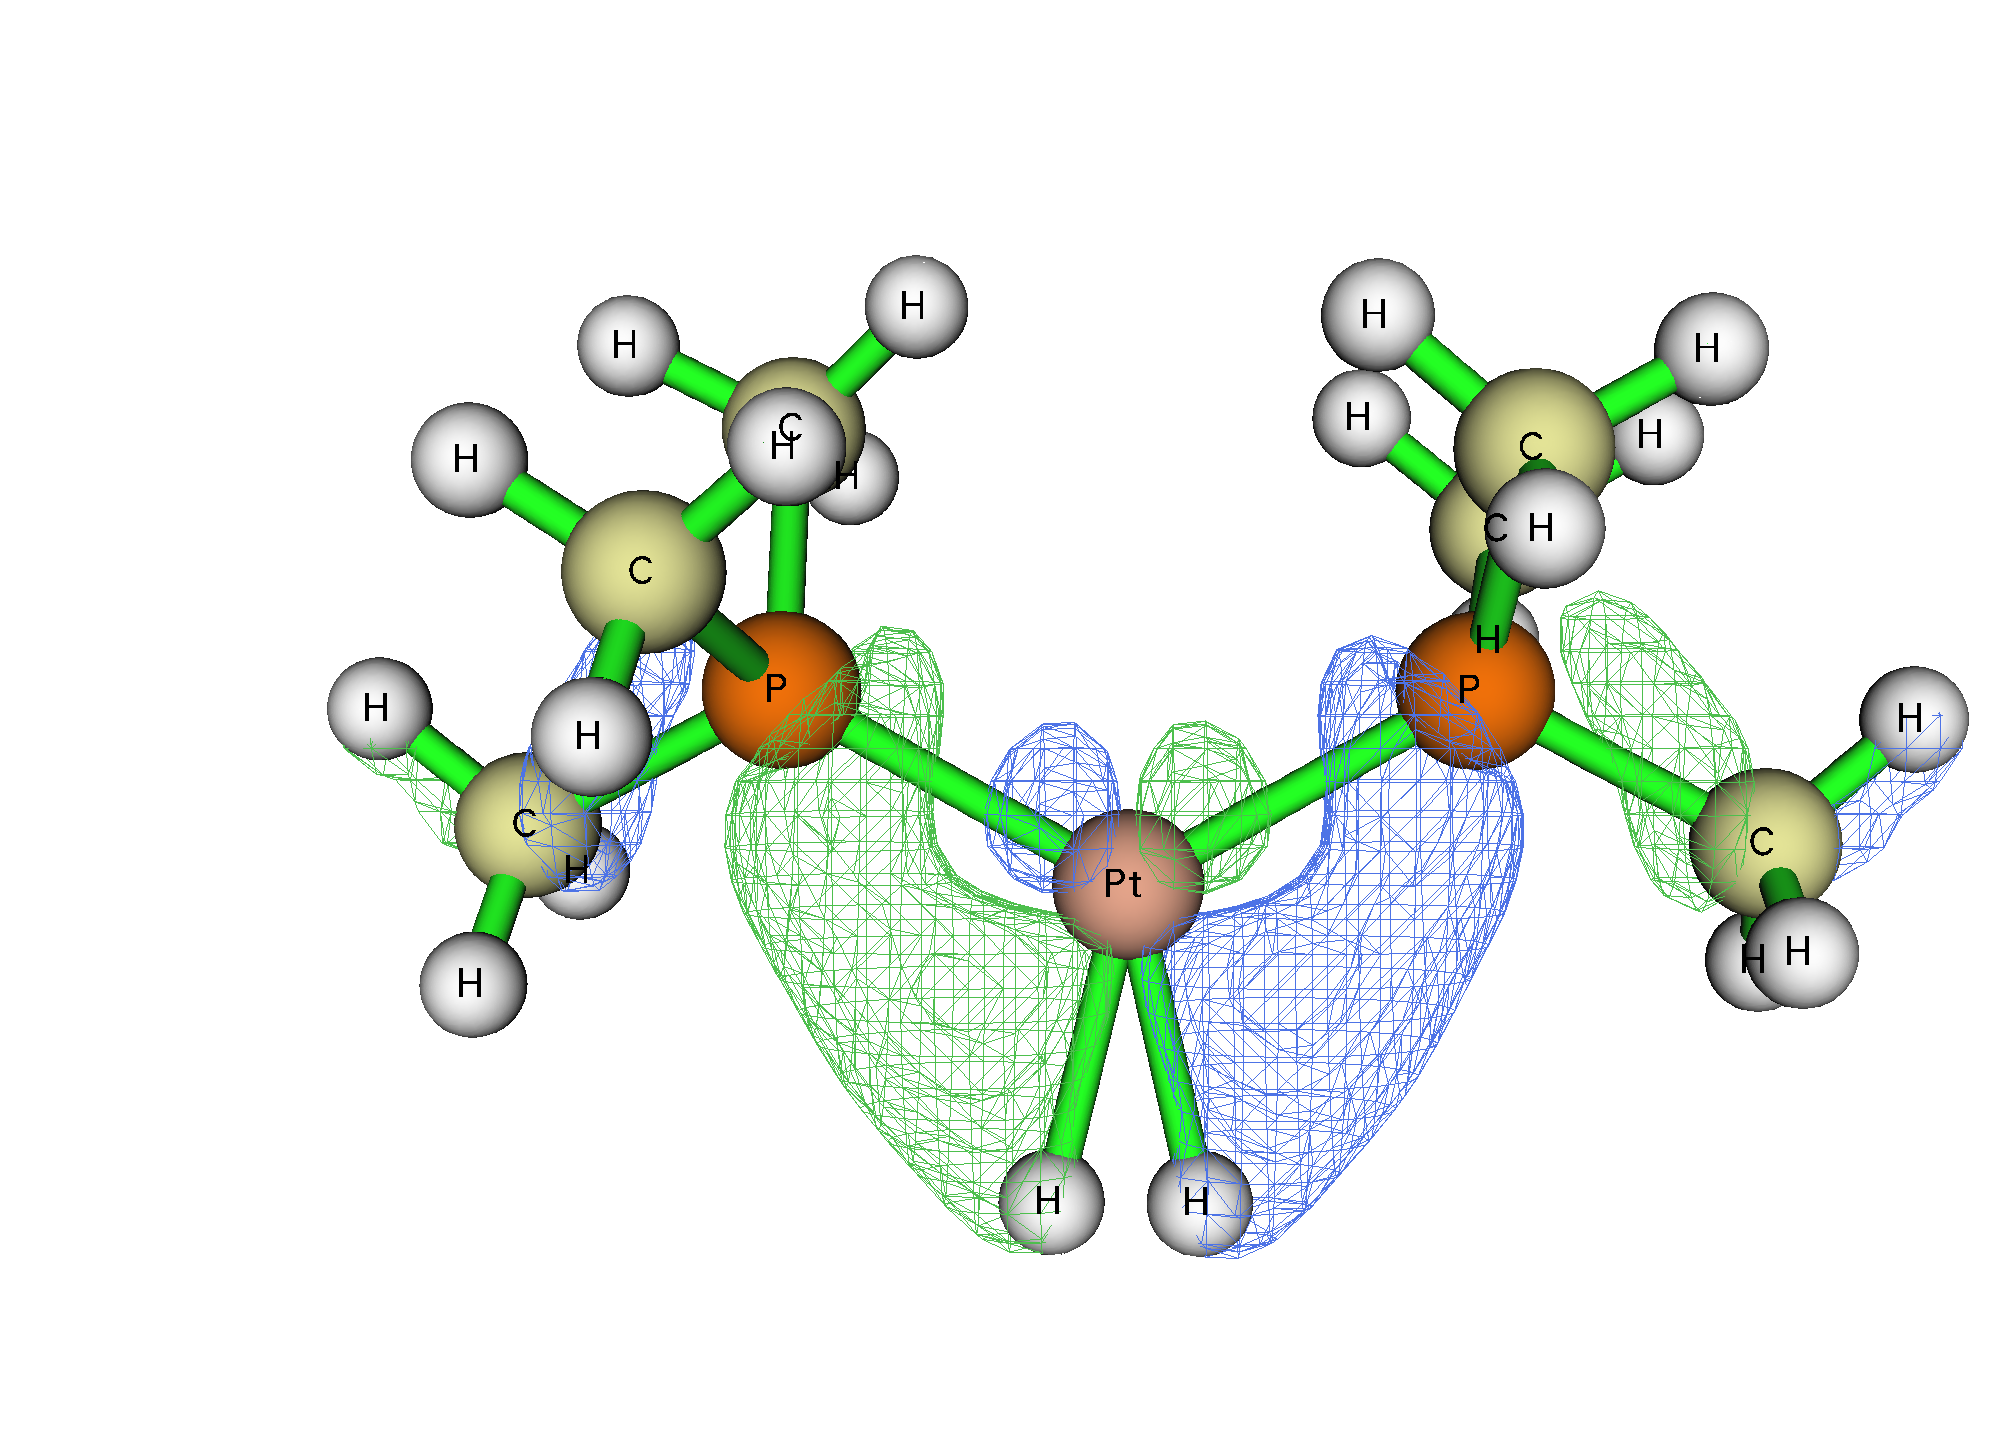
\includegraphics[width=0.45\linewidth]{Pt_tsb_orb.png}
\end{figure}
Calculated at PBE0-D3/def2-TZVP.
\end{frame}

\begin{frame}
%\begin{figure}
%	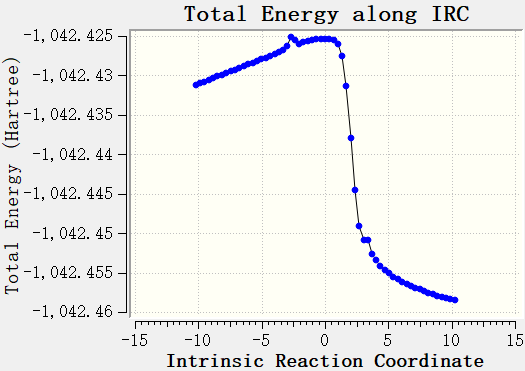
\includegraphics[width=0.45\linewidth]{../Pt/Pt_ircb2.png}
%\end{figure}
Reaction path from literature
\begin{figure}
	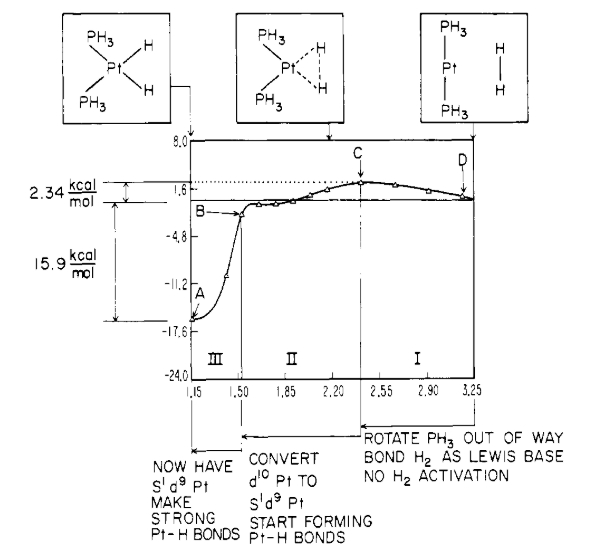
\includegraphics[width=0.48\linewidth]{god1.jpg}
	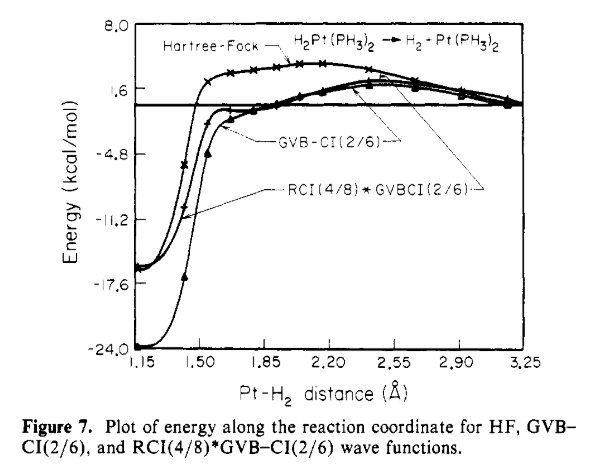
\includegraphics[width=0.5\linewidth]{god2.jpg}
\end{figure}
\fullcite{Goddard1984}
\end{frame}

%\begin{frame}
%"Modern" Solutions:
%\begin{enumerate}
%	\item Do DFT for different spin states, and find MECP
%	\item CASSCF
%\end{enumerate}
%\end{frame}

\begin{frame}
Reaction Path
\begin{columns}
	\column{0.5\linewidth}
	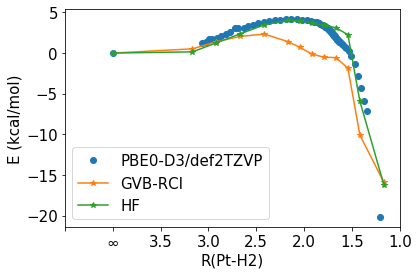
\includegraphics[width=\linewidth]{../Pt/pbe0/irc/irc.png}
    \column{0.5\linewidth}
    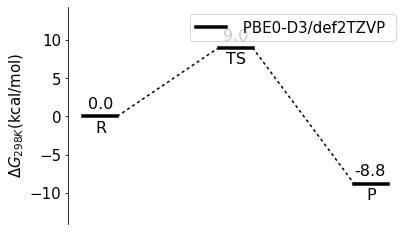
\includegraphics[width=\linewidth]{../Pt/pbe0/Pt.png}
\end{columns}
\begin{table}
	\centering
	\begin{tabular}{ccccc}
		\hline
		& $ R_{\ce{PtH}} $ & $ A_{\ce{HPtH}} $ & $ R_{\ce{PtP}} $ &$ A_{\ce{PPtP}} $\\ \hline
		pre-R & $ \infty $ & - & 2.247 & 180.0 \\
		TS & 2.167 & 20.66 & 2.244 & 148.7 \\
		P & 1.615 & 83.42 & 2.290 & 102.6\\
		%HF & 1.81 & 1.5 &  & pre- \\
		\hline
	\end{tabular}
	\caption{Bond lengts (\AA) and bond angles (\textdegree), at PBE0-D3/def2TZVP}
\end{table}

\textbf{Question}: Do we need triplet and MECP calculation?

%\begin{table}[H]
%	\centering
%	\begin{tabular}{cccc}
%		\hline
%		& R & TS & P \\ \hline
%		$ E_{elec} $(B2PLYPD3/def2-TZVP) &  &  &    \\
%		$ \Delta G_{freq} $(M06-2X/SDD/6-31g*) &  &  &    \\
%		$ \Delta G_{sol} $(M06-2X/SDD/6-31g*) & & & \\
%%	\end{tabular}
%	\caption{Energies}
%\end{table}
\end{frame}

\begin{frame}
\frametitle{Charge Transfer}
\begin{columns}
	\column{0.5\linewidth}
	\begin{figure}
		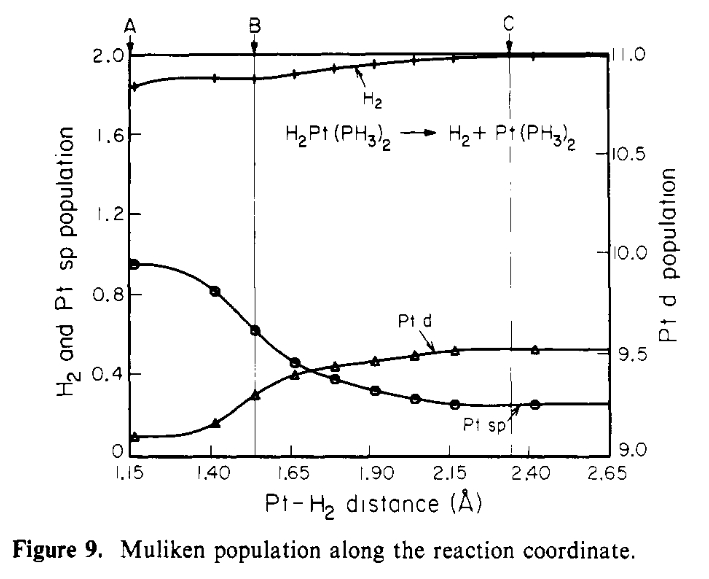
\includegraphics[width=\linewidth]{pop.jpg}
	\end{figure}
    \column{0.5\linewidth}
    \fullcite{Goddard1984}
\end{columns}

Natural Electron Configuration from NBO
\begin{table}
	\centering
	\begin{tabular}{c|ccc}
		\hline
		& R & TS & P \\ \hline
		Pt 5d & 9.51  &9.52& 9.26\\
		Pt 6s & 1.12 &0.91& 0.83\\
		%Pt 6p & & 0.01&\\
		H 1s &   & 1.00& 1.23\\
		%P 3s & 1.24 & 1.26 
		%P 3p & 2.72 & 2.74
		%P 3d & 0.03 & 0.04
		\hline
	\end{tabular}
\end{table}



\end{frame}

\begin{frame}
Natural Bonding
\begin{table}
	\centering
	\begin{tabular}{c|ccc}
		\hline
		& R & TS & P \\ \hline
		Pt-P & $ sd^{0.27}-sp^{1.94}(1.97) $ &  $ sd^{0.13}-sp^{1.94}(1.94) $ & \\	
		Pt-P & $ sd^{0.27}-sp^{1.94}(0.45) $ &  $ sd^{0.13}-sp^{1.94}(0.40) $ & \\
		Pt-H & & & $ sd^{1.10}-s(1.91) $ \\
		Pt-H & & & $ sd^{1.10}-s(0.47) $ \\
		%H 1s &   & 1.00& 1.23\\
		%P 3s & 1.24 & 1.26 
		%P 3p & 2.72 & 2.74
		%P 3d & 0.03 & 0.04
		\hline
	\end{tabular}
\end{table}



\end{frame}
%\section{Reaction III}
%\begin{frame}

% Homework
% 参与反应的轨道
% Pt,Pd,Ni
% 不同构象NBO
% Me->H,CF3

%\printbibliography
%\end{frame}
%\bibliography{icc_pre_1108}
%\bibliographystyle{plain}


\end{document}